\documentclass[a4paper,11pt]{article}
\usepackage[T1]{fontenc}
\usepackage[utf8]{inputenc}
\usepackage[top=1in, bottom=1in, left=0.5in, right=0.5in]{geometry}
\usepackage{amsmath}
\usepackage{graphicx}
\usepackage[superscript,biblabel]{cite}
\usepackage{url}


\title{CS296 Group 09 - Final Project Report}

\author{
  Deepali Adlakha\\
  \texttt{11D170020}\\
  \texttt{dadlakha0111@gmail.com}
  \and
  K. Kartik Pranav\\
  \texttt{110050062}\\
  \texttt{kartikpranav.k@gmail.com}
  \and
  Vibhor Kanojia\\
  \texttt{110050036}\\
  \texttt{versatilevibhor@gmail.com}
}

\date{10th April, 2013}

\begin{document}

\bibliographystyle{plain}

\maketitle

\section*{0 ~~Introduction}
The following is a report of the CS 296 project done by Group 09. We have designed a Rube Goldberg Machine~\cite{rgm}, and implemented our design using the Box2D API in C$++$.\\
Here's our initial design, made using Inkscape:
\\
\begin{center}
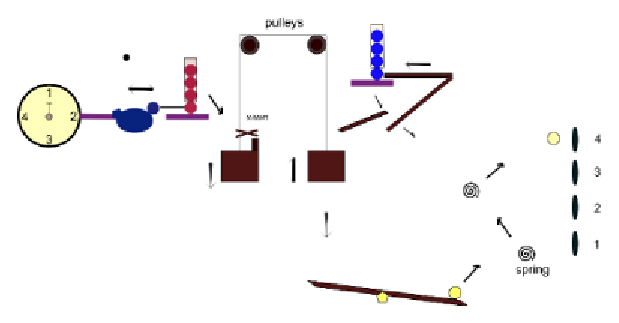
\includegraphics{doc/rgm.eps}
\end{center}
And here's our simulation in Box2D:
\\
\begin{center}
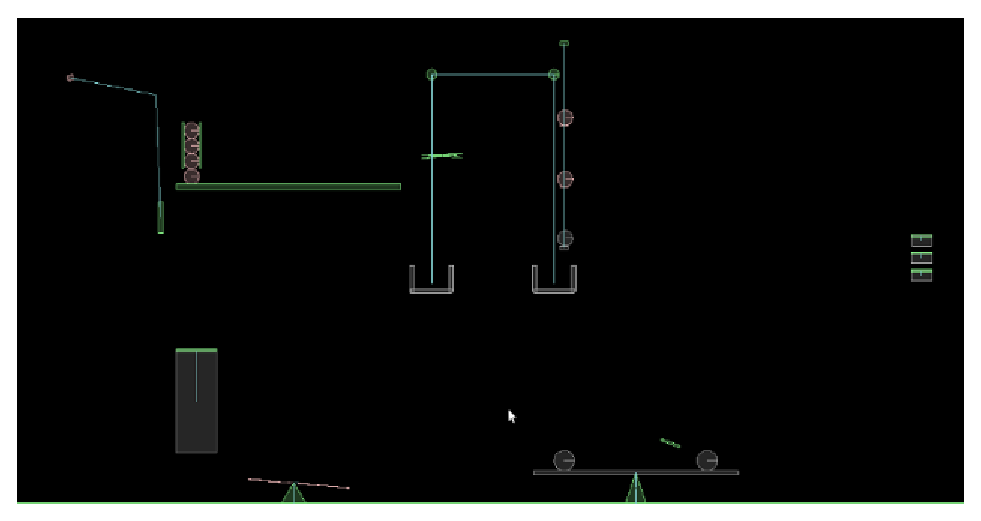
\includegraphics{doc/rgmsim1.eps}\\
\end{center}

Note that we have changed the simulation a little, in place of the 'clock' we had initially, we now have a pendulum that changes its initial angle depending on the case.

\section{The Idea: What's the big deal?}

\subsection{Inspiration}
Representative of election day 2012 in the US, Rube Goldberg himself invented a machine that recorded votes from the general public~\cite{rube-election}:
\\
\begin{center}
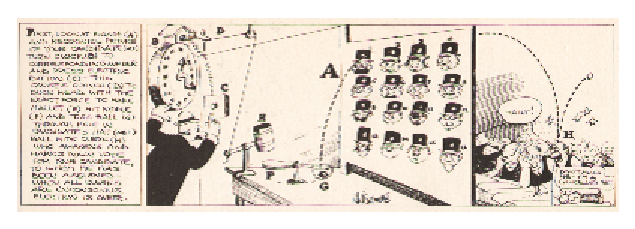
\includegraphics[scale=1.5]{doc/elections.eps}
\end{center}
This was the essesntial idea behind our simulation. The aim - to get a ball to hit one of many different targets depending on initial conditions (in our case, the angle of the pendulum we started out with).

\subsection{Our version}
With this in mind, we used a pendulum to do something similar to what the clock was doing in the above machine. This is because implementing something that moved back and forth wouldn't be as appealing as a pendulum. It also makes it easier to measure time intervals between the falling of the balls into the lefthand- and righthand-side boxes.
\begin{center}
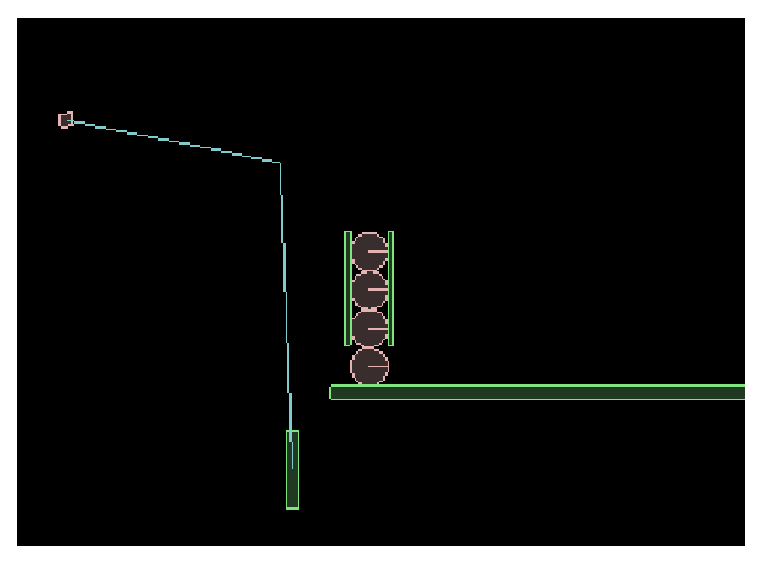
\includegraphics[scale=0.5]{doc/pendulum.eps}
\end{center}

We have also implemented the equivalent of a pair of scissors, which cuts the string tying the boxes together, when the left box rises enough to hit it. For this, we had to create our own contact list of the bodies in Box2D, and our own scissors class, that takes as input the entity it must destroy (i.e. cut the string, in this case) when it comes into contact with it.
\begin{center}
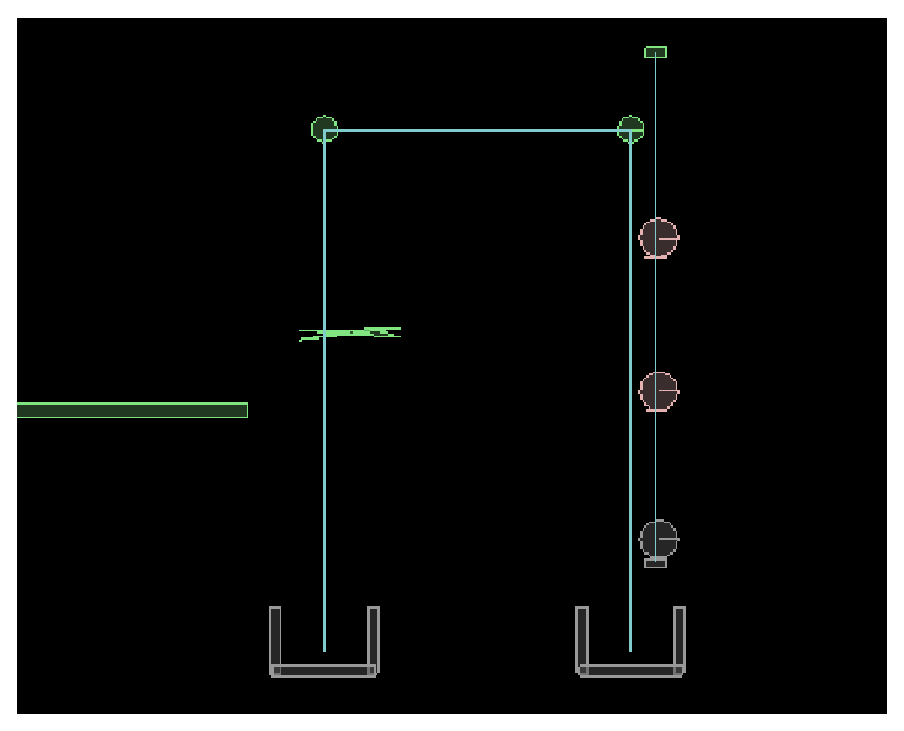
\includegraphics[scale=0.4]{doc/scissors.eps}
\end{center}

A major addition to our design, is that we have added an epilogue-style area, where there are three 'humans' (made of rods, blocks and spheres, at the end of the day) at the other end of the targets. Depending on which target is hit, a pulley system is activated, which eventually causes that person to raise his 'hand.' This makes up for a loss of elements that we weren't able to implement from our original design, and it alo conforms with the election-themed idea we were pursuing. And it looks cool! This part is shown below:

\begin{center}
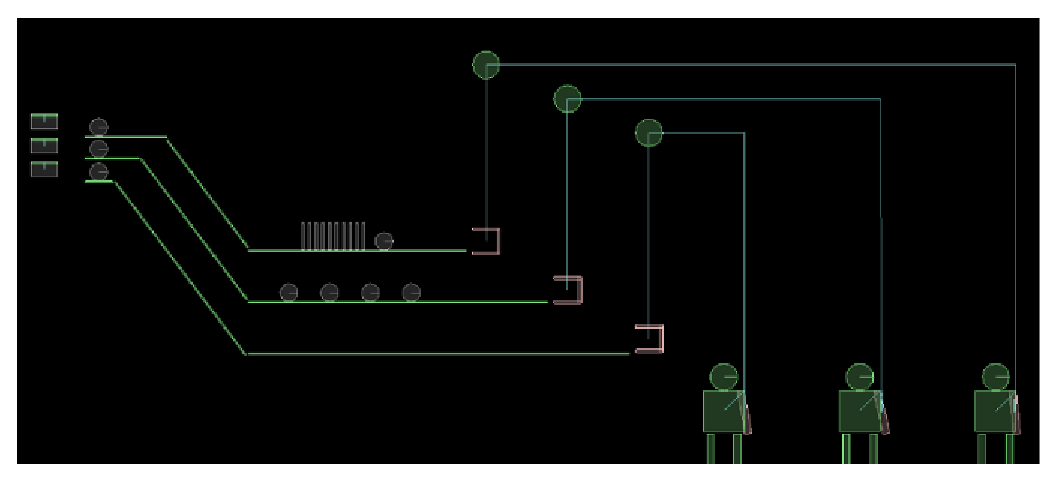
\includegraphics{doc/people.eps}
\end{center}

To select amongst these candidates, we have included an option at the bottom. You can select any one of the three candidates, and their respective hand will shoot up at the end of the simluation.

\begin{center}
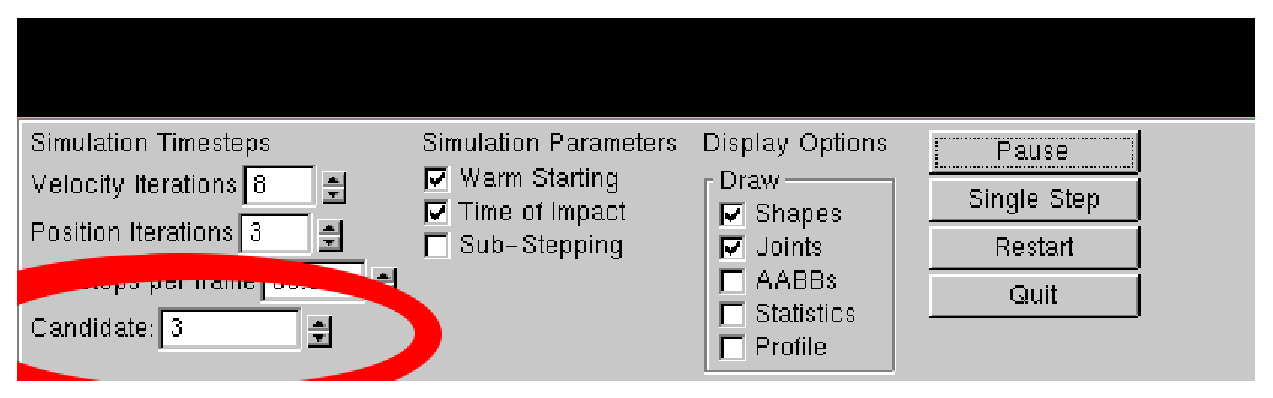
\includegraphics[scale=0.6]{doc/select1.eps}
\end{center}

\section{Analysis of the Code}
\subsection*{The Timing Part}
Similar to an earlier analysis of the base code using profiling and timing, we have plotted 6 graphs depicting the variation of various parameters, after running the executable 100 times for each iteration number (which also runs from 1 to 100). The results of this analysis are shown below:
\\
\begin{enumerate}
  \item Loop time vs. Step time
  \begin{center}
  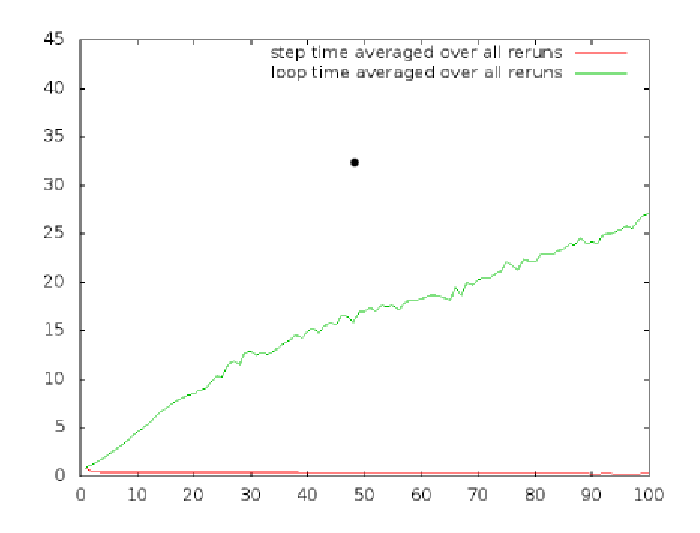
\includegraphics{doc/g09_plot01.eps}
  \end{center}
  The loop time seems to increase almost linearly, or at a minutely slower rate as the step time increases. This is because the loop time is a cumulative sum of step times.

  \item Step time and Update times
  \begin{center}
  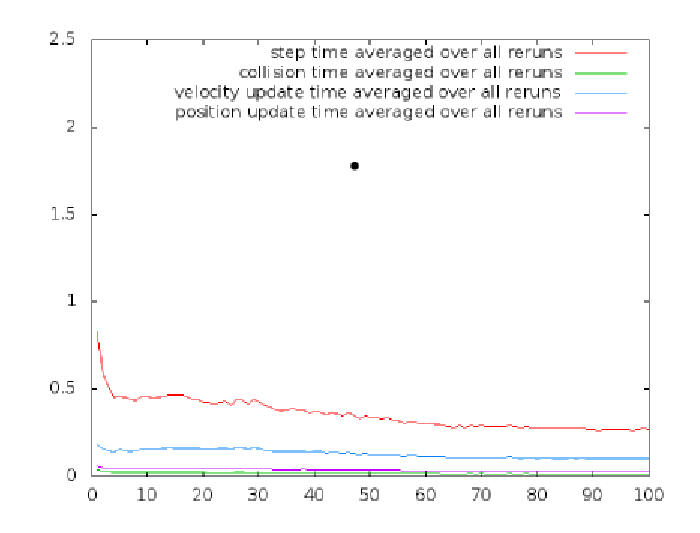
\includegraphics{doc/g09_plot02.eps}
  \end{center}
  The step time must be greater than all the other times, and they all decrease as the iterations increase, due to scheduling and prioritizing of processes.
  
  \item Step time and update times for Reruns
  \begin{center}
  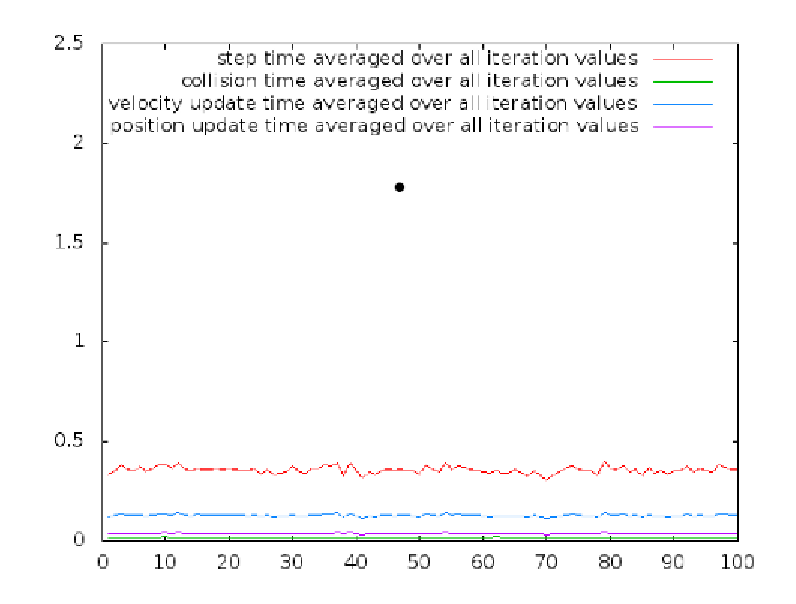
\includegraphics{doc/g09_plot03.eps}
  \end{center}
  Here the number of iterations are constant, so the values obtained remain almost same throughout each rerun.
  
  \item Loop time vs. Step time for Reruns
  \begin{center}
  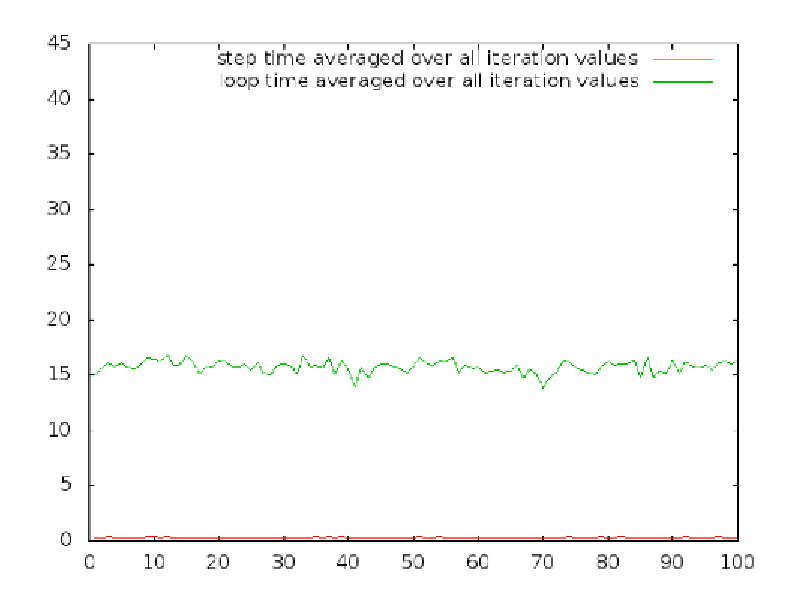
\includegraphics{doc/g09_plot04.eps}
  \end{center}
  Again, the iteration number is kept constant, so not much change is seen across reruns. As usual, the loop time is greater than the step time.
  
  \item Step time with standard deviation
  \begin{center}
  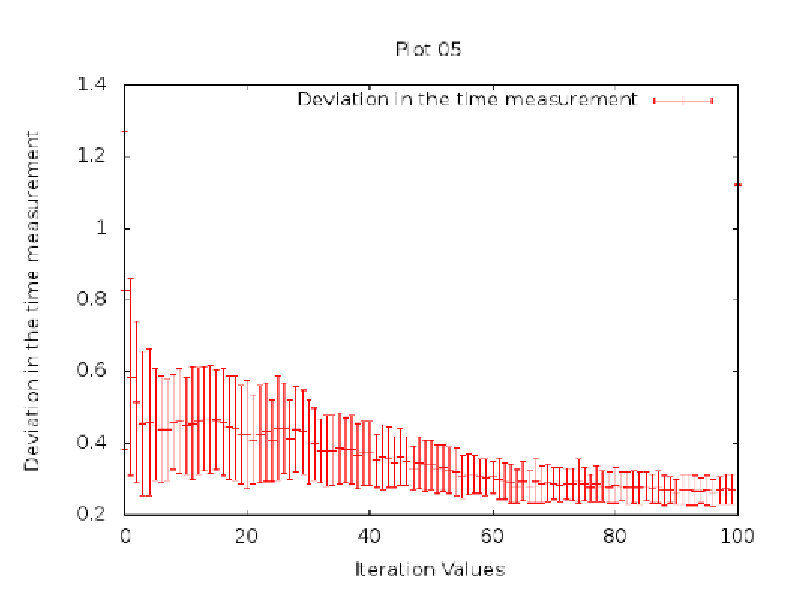
\includegraphics{doc/g09_plot05.eps}
  \end{center}
  The step time decreases over increasing iteration number, as inferred above. The standard deviation progressively decreases in the same way, because with higher iterations, there are more sample points in the space.
  
  \item Cumulative Frequency Bar Graph
  \begin{center}
  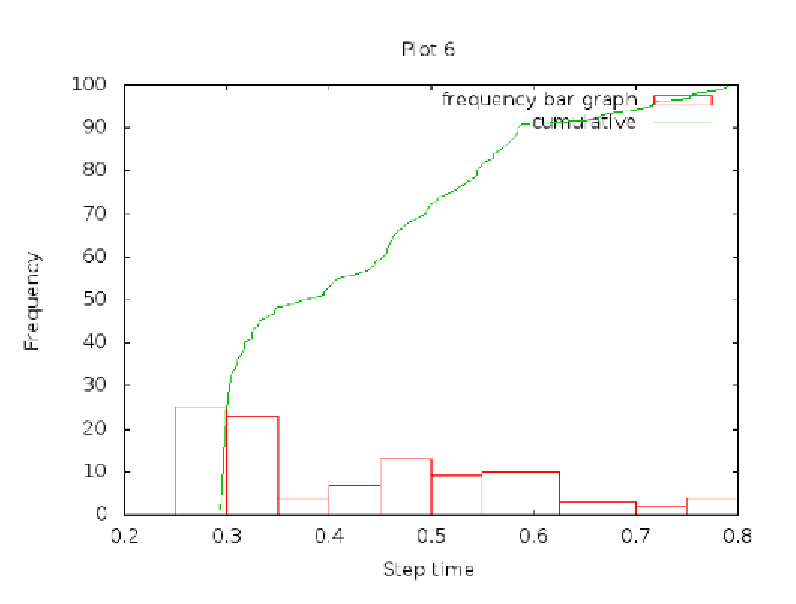
\includegraphics{doc/g09_plot06.eps}
  \end{center}
  Here, we observe the maximum frequency at around 0.3, whereas it would have been at a higher value if the system were loaded. This shows that the process does indeed take more time in the case of a loaded system.
\end{enumerate}

\subsection*{The Profiling and Call Graph}
The call graph represents the time spent in every function, the calling of one function by another, their dependencies etc. We can find the functions that took a large amount of time, those that were called often, and such. This is made much easier when viewed visally, which can be done with the gprof2dot.py Python script ~\cite{py-script}. Here is part of the call graph for the code without optimizations:
\begin{center}
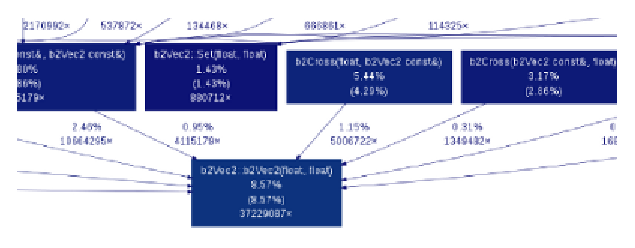
\includegraphics{doc/notopt.eps}
\end{center}
This shows that the function $b2Vec2$ takes a lot of function calls, and this can be improved upon, epsecially with function inlining.\\
When the call graph of the optimized (using $-O3$ flags) is drawn, it appears as a straight line of function names, indicating that there is no dependency of one function on another, i.e. complete function inlining has been done to optimize the code.


\section{Conclusion}
All in all, we have learnt a lot from this project. About the Box2D API (experience with such an API), analyzing and profiling code, and tidbits about C$++$ in general. We also learnt about source version control (using Git, in our case), and most importantly, how to create a distributable version of your source code for public usage. This is something that is in practice in the open-source world today.
\begin{center}
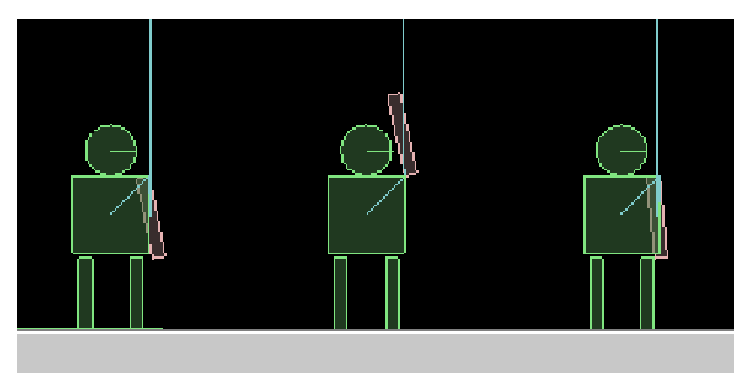
\includegraphics{doc/hello.eps}
\end{center}
\bibliography{doc/ref}
\end{document}
